Wie kann die Energieverteilung des Energieverlustes beschrieben werden? Der Energieverlust ist ein
statistischer Prozess mit einer asymmetrischen Verteilungsfunktion, da Kollisionen mit kleinem
Energieübertrag wahrscheinlicher sind als solche mit großen Energieübetrag.

\begin{figure}[H]
	\centering
	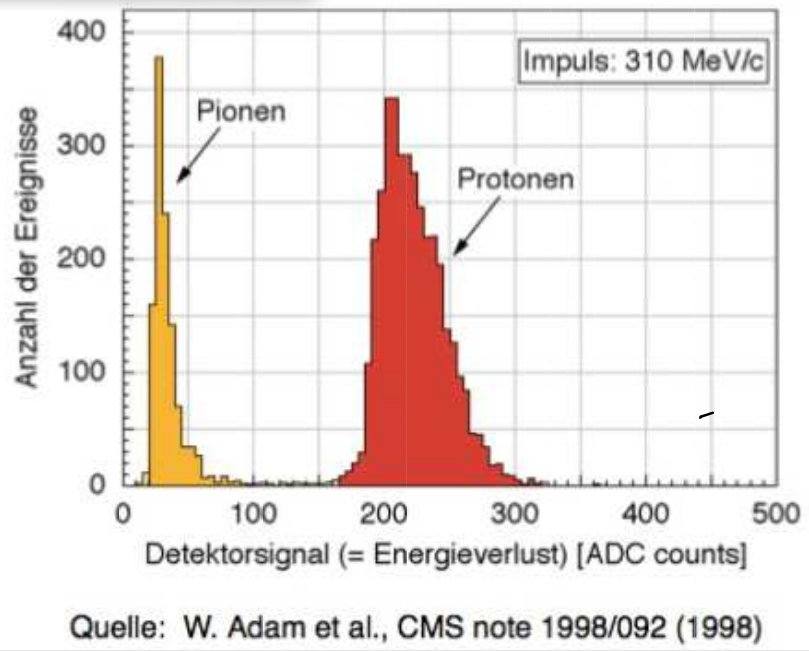
\includegraphics[width=0.5\textwidth]{landau.jpg}
	\caption{Die Energieverteilung des Energieverlustes ist eine Landau-Verteilung.}
	\label{}
\end{figure}

Die Ausläufer bei hohen Energieüberträgen kommt von (selten auftretenden) Kollisionen mit kleinen
Stoßparametern, wobei Elektronen mit großen Energien (keV), sogenannte $\delta$-Elektronen,
freigesetzt werden. Die Asymmetrie kommt daher, dass der mittlere Energieverlust höher
ist als der wahrscheinlichste Energieverlust.
\\
Bei dünnen Absorbern wird der Energieverlust durch eine Landau-Verteilung beschrieben, bei dicken
Absorbern geht diese über in eine Gauß-Verteilung.
